\documentclass[a4paper,11pt]{article}
\usepackage[utf8]{inputenc}
\usepackage[T1]{fontenc}
\usepackage{graphicx}
\usepackage{amsmath}
\usepackage{geometry}
\geometry{margin=2.5cm}

\title{Documentazione della Pipeline Immagini \\ \texttt{xai\_img}}

\begin{document}
\maketitle

\section*{1. Contesto}
Lo scopo principale di questa pipeline è confrontare visivamente e quantitativamente le spiegazioni generate da due diversi metodi di interpretabilità su immagini analizzate da modelli di machine learning. Nello specifico, si vogliono identificare e quantificare eventuali differenze significative (\emph{Disagreement Problem}) tra le regioni dell'immagine che i diversi metodi considerano più importanti per la decisione del modello.

In pratica, dati:
\begin{itemize}
\item una rete neurale pre-addestrata (ResNet-18);
\item una singola immagine ( in questo caso la foto di un gatto);
\item due metodi di interpretazione (Integrated Gradients e Saliency);
\end{itemize}
la pipeline produce due mappe di salienza, che rappresentano visivamente le zone dell'immagine considerate determinanti per la classificazione. Successivamente, confronta queste mappe usando metriche numeriche per stabilire se e quanto queste spiegazioni divergano tra loro.

Questo confronto aiuta a comprendere se metodi diversi offrono una visione coerente o se, al contrario, identificano regioni diverse come importanti, generando potenziale confusione o difficoltà nell'interpretazione delle decisioni del modello.

\section*{2. Tecnologie e librerie}
È stato utilizzato Python 3.10 in ambiente \texttt{anaconda (xai)}, con:
\begin{itemize}
\item \textbf{PyTorch} e \textbf{torchvision} per il caricamento della rete pre-addestrata;
\item \textbf{Captum} per i metodi di interpretazione;
\item \textbf{scikit-image} per la segmentazione in super-pixel;
\item \textbf{NumPy} per la gestione delle mappe di salienza;
\item \textbf{Matplotlib} per la visualizzazione grafica dei risultati.
\end{itemize}

\section*{3. Metodi di interpretazione}
I metodi di interpretazione sono tecniche che ci permettono di capire "perché" un modello di intelligenza artificiale ha preso una certa decisione. In questo caso, lavoriamo con immagini e vogliamo sapere quali zone dell'immagine hanno influenzato maggiormente la classificazione del modello.

\subsection*{3.1 Integrated Gradients (IG)}
Integrated Gradients è un metodo che cerca di spiegare l'importanza di ciascun pixel di un'immagine. Funziona così:
\begin{itemize}
\item si parte da un'immagine completamente nera (nessuna informazione);
\item si calcola gradualmente quanto ogni pixel dell'immagine reale cambia il risultato del modello mentre "si accende" (cioè mentre passa da nero al suo valore reale);
\item si sommano tutti questi piccoli cambiamenti per ogni pixel.
\end{itemize}
Il risultato è una mappa in cui ogni pixel ha un valore che indica quanto ha influenzato la decisione.

Più è alto il numero di passi (\texttt{n\_steps}), più precisa è la stima, ma il calcolo richiede più tempo.

\subsection*{3.2 Saliency (gradiente puro)}
Saliency è un metodo molto più semplice. Calcola direttamente quanto la predizione del modello cambierebbe se modificassimo leggermente ogni singolo pixel. Più il cambiamento è grande, più quel pixel è importante.

Differenze principali rispetto a IG:
\begin{itemize}
\item \textbf{Veloce}: richiede un solo calcolo;
\item \textbf{Rumoroso}: spesso mette in evidenza molti pixel sparsi, anche se non sono realmente importanti;
\item \textbf{Non richiede baseline}: non parte da un'immagine nera.
\end{itemize}


\section*{4. Flusso di lavoro}
La pipeline è suddivisa in due fasi principali: creazione delle mappe e confronto tra di esse.

\subsection*{4.1 Creazione delle mappe (\texttt{make\_maps.py})}
Questa fase genera due mappe di salienza, una con Integrated Gradients e una con Saliency:

\begin{enumerate}
\item \textbf{Caricamento modello}: si utilizza ResNet-18 pre-addestrata su ImageNet.
\item \textbf{Caricamento immagine}: l'immagine (es. \texttt{cat.jpg}) viene ridimensionata a 224x224, convertita in tensore e normalizzata secondo lo standard del modello.
\item \textbf{Integrated Gradients}:
\begin{itemize}
\item si definisce una baseline nera (immagine completamente vuota);
\item si calcola l'importanza di ogni pixel seguendo il metodo IG;
\item si somma sui canali e si salva la mappa come \texttt{saliency\_A.npy}.
\end{itemize}
\item \textbf{Saliency (gradiente puro)}:
\begin{itemize}
\item si calcola direttamente il gradiente rispetto all'immagine;
\item si somma sui canali e si salva la mappa come \texttt{saliency\_B.npy}.
\end{itemize}
\end{enumerate}

Alla fine, il file stampa:
\begin{verbatim}
saliency_A.npy e saliency_B.npy salvati.
\end{verbatim}

Questi due file contengono le mappe da confrontare nella fase successiva.

\subsection*{4.2 Confronto delle mappe (\texttt{compare\_saliency.py})}
Questa fase serve a confrontare quantitativamente le due mappe generate, per capire se evidenziano le stesse regioni dell'immagine oppure no.

\begin{enumerate}
\item \textbf{Caricamento delle mappe e immagine}: le due mappe salvate vengono caricate. L'immagine originale viene ridimensionata per avere la stessa dimensione delle mappe.

\item \textbf{Segmentazione in super-pixel (SLIC)}:
L'immagine viene divisa in 200 "super-pixel" tramite l'algoritmo SLIC, cioè piccoli blocchi omogenei di pixel simili. Ogni blocco avrà un'etichetta diversa.

\item \textbf{Creazione dei vettori di salienza}: per ciascun super-pixel si calcola la media dei valori di salienza. Si ottengono così due vettori (uno per ogni mappa), che rappresentano l'importanza media di ciascun blocco.

\item \textbf{Metriche di confronto}:
Si calcolano quattro misure che quantificano il disaccordo tra i due vettori:
\begin{itemize}
\item \textbf{FeatureDisagreement}: misura quanta sovrapposizione c'è tra i blocchi più importanti nelle due mappe.
\item \textbf{SignDisagreement}: come sopra, ma tiene conto anche del segno (positivo o negativo).
\item \textbf{Euclidean}: distanza globale tra i due vettori (con segno).
\item \textbf{Euclidean-abs}: distanza globale tra i due vettori, ignorando il segno.
\end{itemize}
Il parametro \texttt{K\_FRAC = 0.05} indica che si considera il top 5\% dei super-pixel più importanti.

\item \textbf{Visualizzazione}:
Viene creato un overlay che mostra l'immagine originale affiancata dalle due mappe colorate. I colori indicano l'importanza: rosso = alta, blu = bassa.
\end{enumerate}

Il programma stampa a video i quattro valori numerici delle metriche e mostra graficamente le differenze tra le due spiegazioni.

\section*{5. Risultati}
Eseguendo:
\begin{verbatim}
python make_maps.py
python compare_saliency.py
\end{verbatim}
si ottiene:
\[
\begin{aligned}
\text{FeatureDisagreement} &= 1.000,\\ 
\text{SignDisagreement}    &= 1.000,\\
\text{Euclidean}           &= 1.417,\\
\text{Euclidean-abs}       &= 0.856.
\end{aligned}
\]
Questi valori indicano disaccordo massimo sulle top‐5\% di super‐pixel e grande distanza globale, confermando che le due mappe (IG vs Saliency) evidenziano aree significativamente diverse.

\subsection*{5.1 Interpretazione quantitativa}
\begin{itemize}
\item \textbf{FeatureDisagreement = 1.000}: fra i super‐pixel “top‐k” scelti da saliency A e quelli scelti da saliency B, non c’è alcuna sovrapposizione (100\% di disaccordo).
\item \textbf{SignDisagreement = 1.000}: anche considerando il segno dell’attribuzione (positivo vs negativo), non c’è alcuna corrispondenza nelle stesse regioni.
\item \textbf{Euclidean $\approx$ 1.417}: misura “globale” di distanza $L_2$ fra le due distribuzioni di saliency (vettori normalizzati): quindi le due mappe sono molto diverse.
\item \textbf{Euclidean‐abs $\approx$ 0.856}: stessa distanza ma ignorando il segno: resta elevata, il che conferma che anche le intensità “in assoluto” sono molto differenti.
\end{itemize}

\section*{6. Le tre immagini}
\begin{figure}[htbp]
\centering
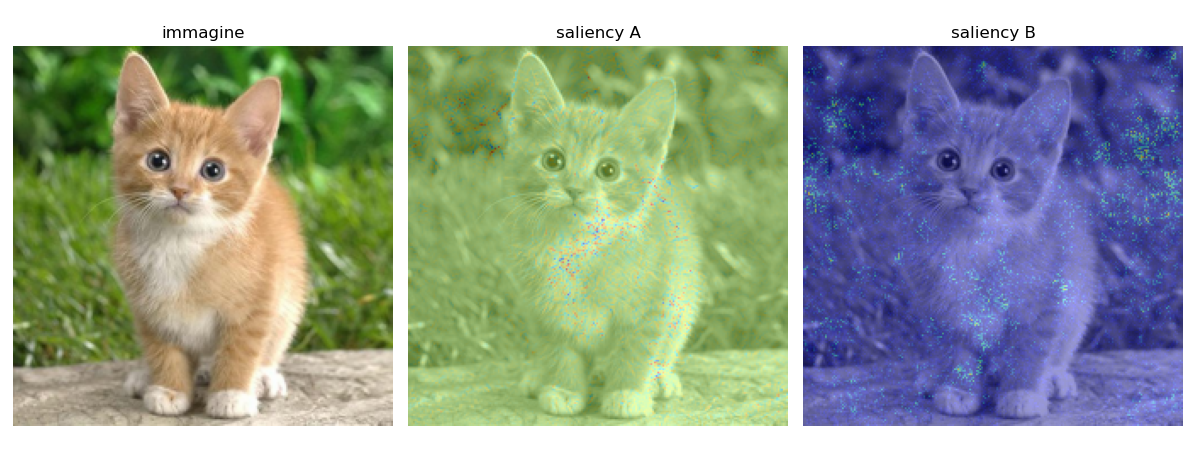
\includegraphics[height=3.5cm]{saliency.png}\qquad
\caption{Da sinistra: immagine originale, heat‐map IG (saliency A), heat‐map Saliency (saliency B).}
\label{fig:three_images}
\end{figure}

\subsection*{6.1 Immagine originale}
La foto originale (\texttt{cat.jpg}), ridimensionata a 224×224 pixel per coincidere con le mappe.

\subsection*{6.2 Saliency A}
Overlay della mappa generata con Integrated Gradients. I colori (scala dal verde al rosso, mappati con \texttt{plt.cm.jet}) mostrano le aree che IG ritiene importanti: più una zona è “rossastra”, più pesa sulla decisione del modello. Qui emerge una colorazione diffusa, con pochissime aree calde concentrate.

\subsection*{6.3 Saliency B}
Overlay della mappa generata con il metodo Saliency (gradiente puro). Qui il colore prevalente è bluastro, con pochi puntini verde‐chiaro che indicano dove il gradiente è massimo.

\section*{7. Discussione sul Disagreement Problem}
Nessuna sovrapposizione nelle aree top‐k (FeatureDisagreement = 1) → IG e gradiente puro indicano regioni completamente diverse come “più importanti”.

Anche le intensità complessive non sono vicine (Euclidean = 1.417) → l’intero pattern di saliency è distante.

Visivamente, IG ha evidenziato una zona ampia e sfumata (al centro del manto), mentre Saliency ha punti sparsi in tutta l’immagine.

Due explainers, applicati allo stesso modello e alla stessa immagine, raccontano storie molto diverse su quali pixel abbiano spinto la predizione.

\section*{Glossario}

\begin{itemize}
  \item \textbf{Salienza (saliency map)}: immagine che mostra quali parti dell’immagine originale hanno contato di più nella decisione del modello.
  \item \textbf{Gradiente}: misura di quanto cambierebbe il risultato del modello se modificassi appena il valore di un pixel (quanto “sensibile” è il modello a quel pixel).
  \item \textbf{Integrated Gradients}: tecnica che valuta l’importanza di ogni pixel sommando il contributo dei gradienti mentre l’immagine passa da vuota a reale.
  \item \textbf{Super-pixel}: gruppi di pixel simili tra loro, trattati come blocchi per semplificare il confronto tra mappe.
  \item \textbf{Heatmap}: rappresentazione visiva con colori, dove ad esempio il rosso mostra le zone importanti e il blu quelle meno importanti.
\end{itemize}


\end{document}
